\documentclass[12pt,a4paper]{article}

\renewcommand{\baselinestretch}{2} 
\usepackage[margin=1.0in]{geometry}

\usepackage{amsmath}
\usepackage{amssymb}
\usepackage{relsize}
\usepackage{graphicx}
\usepackage{verbatim}
\usepackage{hyperref}
\usepackage{relsize}
\usepackage{amsthm}

\usepackage{pgffor}%
\usepackage{geometry}
\usepackage{pdflscape}

\usepackage[utf8]{inputenc}
\usepackage[english]{babel}

\newtheorem{theorem}{Theorem}[section]
\newtheorem{lemma}[theorem]{Lemma}
\newtheorem{proposition}[theorem]{Proposition}
\newtheorem{corollary}[theorem]{Corollary}
\newtheorem{assumption}[theorem]{Assumption}


\newenvironment{definition}[1][Definition]{\begin{trivlist}
\item[\hskip \labelsep {\bfseries #1}]}{\end{trivlist}}
\newenvironment{example}[1][Example]{\begin{trivlist}
\item[\hskip \labelsep {\bfseries #1}]}{\end{trivlist}}
\newenvironment{remark}[1][Remark]{\begin{trivlist}
\item[\hskip \labelsep {\bfseries #1}]}{\end{trivlist}}

\begin{document}


\title{Impacts of Taxes on Firm Entry Rates along State Borders}
\author{Kevin D. Duncan}
\date{}
\maketitle

\begin{abstract}
This paper uses a regression discontinuity approach to estimate the impacts of taxes on firm entry rates between neighboring states. We utilize matched county pairs as an approximate bandwidth around the discontinuity in state policies imposed at their border. This controls for unobserved location specific determinants of firm entry, as well as policy responses to shocks shared across borders. We then estimate the impacts of property, income, sales, corporate, capital gains, workers compensation, and unemployment insurance top marginal tax rates on the differences in firm entry between counties. Our array of taxes controls for joint changes in tax policy that governments may implement to accomplish policy goals. We estimate this impact using a sample of 107 state-border pairs between 1999 and 2009. Our results indicate that property and sales taxes have the largest negative effect on firm start up rates, and in more recent year's income taxes as well.
\end{abstract}

\newpage

\section{Introduction}

Each year states and counties try to incentivize new business start-ups in their locale over alternative choices. The most visible cases include governments offering firm's temporary reprieve from tax burdens, or deals to build infrastructure to support new entrants. There has been a growing literature addressing the efficacy of these exemptions both to state revenue and public welfare. States may also take a long run approach to incentive new firm start-ups by altering their tax and regulatory codes for all market participants. 

This paper tests whether or not taxes impact firm entry rates between neighboring states. We also explore whether or not firms place preferences over government expenditures in their entry decision. This later situation would imply that increasing taxes to pay for certain services may not have distortionary effects on firm start up rates. The paper tests the impacts of seven top marginal tax rates, including property, income, corporate, capital gains, sales, workers compensation, as well as unemployment insurance, and state expenditures per capita on welfare, highways, and education.

We provide two methods to address these problems. We first estimate count data models of firm entry as a benchmark against existing literature in the field. We then outline our preferred estimator, which uses matched county pairs on either side of a state border. By matching counties, we get an approximate bandwidth around the sharp discontinuity in policies at state borders. The process may control for unobserved variables in count data models, as well as interaction terms between policy and location specific components of firm entry. This gives us the ability to identify just the policy effect.

This county-pair difference estimator is a generalization of the traditional difference in difference estimator extended over a larger panel of agents and time periods. It has been used to explore how different policy regimes affect local migration between geographic entities (McKinnish (2005) (2007)), as well as how differences in policies impact outcomes across borders (Holmes (1998), Rohlin (2011), Dube et al (2010), McPhail, Orazem, Singh (2010), Dhar and Ross (2012),  Kahn and Mansur (2013)). Many of these papers focus on how firms or individuals respond to imposed opportunity costs in location from neighbor's policy action.

Broader economic theory provides mixed outcomes to if a higher number of firm start ups increases welfare. Cases where more firms are welfare decreasing appear when assuming fixed costs to entry, such that too many firms entering can exceed their marginal benefit. Comparably if consumers have preferences over differentiated products, increasing the number of firms ('varieties') can be welfare increasing. The theory we develop here works outside of these considerations. Instead our results can help governments achieve higher employment growth and government revenues, as well as extending existing determinants of firm sorting.

The paper proceeds in the following manner. First, we review literature relating to empirical firm sorting and entry and how regression discontinuity techniques have been used in related studies. We then provide a model to show why state borders may allow us to control for location specific terms of firm entry. Next, we explain our empirical design, which uses both count data models  and a regression discontinuity technique using matched county pairs. Finally, we estimate reduced form models of the impact of various policies on firm start up rates. We then provide estimates for the impacts of taxes and government expenditures on firm entry into US counties. We conclude by showing which borders have the largest firm start up discrepancy, and talk about applications and limitations for our work.

\section{Literature Review}

Location choice of firms and individuals has a rich history in economics. At its core, the question is what drives households and firms to choose to locate in particular communities. Tiebout (1956) argued that individuals sorted into locations based on their preferences for prices and public amenities. He posited that, because households can “vote with their feet,” counties have incentives to adjust their provision of services in order to attract residents.\footnote{Sorting literature similarly gave birth to tax competition among states as over viewed by Wilson (1999). Our paper can be seen as an extension of this literature, where states compete to have preferential tax differentials compared to neighboring states}

Guided by Tiebout’s model, the early firm entry literature focused on sorting over all available possible markets.  McFadden (1974) provided a general framework for using the conditional Logit function to estimate firm entry choices over all available possible markets. Early papers such as Carlton (1979, 1983) and Schmenner (1975, 1982) failed to find incidence of taxes on firm entry rates, instead finding that higher taxes could attract more firms. Starting in the 80's methods and data allowed for cleaner identification, such that authors started to more definitively show that taxes had an impact on business activity, including Wasylenko \& McGuire (1985), Bartick (1985), Papke (1991), and Hines (1996).

Researchers have continued to estimate models of firms sorting over a large number of counties. Gabe and Bell (2004) used Poisson and Negative Binomial regressions show how taxes and government spending on education impact firm location in Maine. Their results show that increasing tax rates to raise education spending per pupil causes no distortion on firm entry rates. A review of these sort of sorting estimates was done by Arauzo-Carod et al (2010). In their review they show that agglomeration and market size tend to have a significant positive effect, while wages and taxes act in the opposite direction. Further, the findings on the effect of property values as is implied in the traditional Tiebout models is even weaker (see Dowding, John, and Biggs (1994) for a comprehensive review of Tiebout model estimates).

Increasingly researchers have utilized border-difference technique to establish local estimates of the impacts of taxes on firm entry rates. This method controls for endogeneity of government policy in response to local economic outcomes. For example, high economic activity states may raise their taxes knowing that local agglomeration factors will continue to attract an asymmetrically high amount of new firm start ups, while low economic activity states may lower taxes to attract new businesses.\footnote{Further, tax and other policy parameters tend to feature prolonged periods of stability, and changes may be endogenous to many common dependent variables, such that changes in GDP, wages, and employment will entice government officials to try and improve economic performance. This has led to time series applications to use narrative approaches to try and identify the impacts of exogenous shocks to tax rates on macroeconomic variables. This is why narrative approaches are currently common in the macoreconometrics literature as a way of estimating the impacts of taxes see Romer and Romer (2007), and Mertens and Ravn (2013).} This response would upwards-bias the estimate of the impacts of taxes. Using the differences in firm entry rates along state borders controls for local agglomeration factors, and treat differences in policy variables as exogenous.

This technique relies on the assumption that new firms pick entry locations within a local choice set. Recent studies on agglomeration economies seem to support this view.  Rosenthal and Strange (2003, 2005), and Arzaghi and Henderson (2008)) show that entrepreneurs weight potential locations within a mile of their current location significantly higher than distances further away. Use of border discontinuity designs started with Holmes’ (1998) analysis of right to work laws on manufacturing employment growth. In Holmes' paper, he uses right to work status as a proxy for an unobserved cost of being on either side of a state border imposed by "pro" and "anti" business policies. He then tested whether or not right to work status affected manufacturing employment growth. His estimates found that counties that have right to work status attract more manufacturing firms than states without right to work status.

Since Holms's study, this technique has been adopted by researchers looking to identify effects of additional state policies, including minimum wages (Dube et al, 2008; Rohlin, 2011), welfare (McKinnish, 2005; 2007), and school quality (Dhar and Ross, 2012). Recent papers looking at the impacts of taxes on firm start up rates, including Rathelot and Sillard (2008), Duranton et al (2011), and Rohlin, Rosenthal, and Ross (2014). 

Rohlin (2011) looked at the impact of minimum wages on firm start up rates using aggregated data. By utilizing the Dun and Bradstreet Marketplace data files Rohlin constructed bands around state borders, and then derived estimates on the impact of minimum wage changes on firm start up rates. He showed that increasing the minimum wage decreased new establishment activity in industries that relied heavily on minimum wage workers, but that changes in the minimum wage did not decrease employment in existing establishments. 

Chirinko and Wilson (2008) use a border discontinuity technique to estimate the impact of state investment tax credits on firm start up rates. Rathelot and Sillard (2008) use the border discontinuity technique in a Probit model to show that increasing the total tax rate differential increases the probability of a firm picking a side between 1-5\%. Duranton, et al (2011)  difference firm entry rates in neighboring areas to estimate the impact of taxes on employment. While their  traditional OLS estimates (without the spatial difference)  show a positive relationship between taxes and firm entry rates, after applying the spatial difference, taxes negatively impact firm start up rates. 

A recent paper by Rohlin, Ross, and Rosenthal (2014) mirrors our paper very closely. They estimate a linear probability model of firm entry using a border difference estimator. They use GIS coded data to get a closer bandwidth to the border than our method, and show that increasing the personal income tax differential actually increases the likelihood of firms entering on one side of the border. However, they show that increasing the corporate and sales tax differential can drastically reduce the relative firm entry probability.

Rohlin et al utilize a measure of state-level government expenditures per capita, and utilize Tax Foundation data on top marginal sales, corporate, and personal income tax rates from 2000 to 2003. They estimate a linear probability model of the chance that a firm enters onto one side of the border. They then use reciprocal agreements on where individuals pay income taxes based on location of work rather than location of residence to try to control for proper allocation of tax burdens on each side of the state, and to provide additional strength in identification. Finally, they then use zip code level data to estimate average entry along each side of the border. Both with and without the reciprocal agreements in place, they show that there is a negative impact of increasing the tax differential between states on the probability of firm entry.

Our paper differs by having a considerably larger number of tax policy variables, thus better controlling for other tax policies that may be impact business activity. Moreover, we also include a longer time series than Rohlin et al, providing additional variation in state level tax policies over our window. We differ in only having county level data, rather than the finer zip code level data that Rohlin et al use. This provides a much finer bandwidth to identify the impacts of changes on.

A major issue with the existing literature is the failure to settle on the best variables to use for identifying the effects of taxes on firm start up rates. Carlton (1983) used top marginal tax rates for corporate and income tax, but weighted them together, as well as property tax rates. Schmenner (1987) uses state and local property tax revenues per dollar of personal income. Helms (1985) used a budget constraint to estimate the impacts of rising tax revenue on explanatory variables. All three versions have modern equivalents and the literature has not settled on a single best practice to recover the proper marginal effects.

Theory indicates that marginal tax rates are what matter to individuals, and measures of average tax burden change due to both fluctuations in wages or profits, as well as to changes in tax rates. Using average tax rates may add endogeneity into models. Also, politicians may alter multiple taxes at once in order to accomplish policy goals, such that excluding taxes may imply omitted variable bias. Therefore, we argue that using top marginal tax rates is the preferred method of estimating marginal effects of taxes. 

From the literature, we see that on average taxes negatively impact firm start up rates, especially as researchers have gone from studying sorting over all available entry choices, to local choices along policy discontinuities. However, how taxes are calculated and used in studies differs wildly among authors. Various studies have used measures of average tax revenue, added together top marginal tax rates, or included a single available tax rate. As a result, we employ more recent spatial difference techniques to get a clear estimate, while employing a larger array of top marginal tax rates than other authors.
\section{Theory}

As entrepreneurs and firms look to start up a business in a new location they first choose a market to enter. This choice is due to primary considerations such as labor market characteristics, or location preferences of the owner. They then pick among possible locations in that market. Our model looks at choice of firm entry across state borders, such that individuals have mobility across the border. As a result, firms treat location specific determinants of profit as the same on both side of the border. This process leaves policy drivers as remaining difference in expected profits. We formalize the conditions for this process below.

Assume there exists a spatial equilibrium where wages and capital costs are adjusted to local tax and location specific variables affecting firm level productivity. If markets are competitive firms will make zero economic profit in the long run, but in the short run demand or policy shocks can leave short run profits. We expect that if a regime changes its taxes over time, higher production costs and lower profits exist in that county, and that market will deter a relative amount of firms from entering. Since firms will bid up or down prices relative to taxes, those prices can be proxied by the tax rates directly. Firms make decisions based on information from the previous year, as governments might concurrently change policy along with market entry and there may exist costs to establishing a business.

\begin{assumption}
Assume that a firms' profit can be expressed as a linear function, for a given location, state, and time pair denoted $(i,j,t)$,
\begin{equation}
\pi_{i,j,t} =  \gamma+\beta_{i}+\beta_{j}+X_{i,t-1}\beta_{1}+X_{j,t-1}\beta_{2}+\epsilon_{i,j,t}
\end{equation}
\begin{equation}
E[\epsilon_{ijt}] = 0
\end{equation}
$X_{i,t-1}$ is a $1 \times K_{1}$ row vector of location specific terms, and $X_{j,t=1}$ is a $1 \times K_{2}$ row vector of state specific terms, and $\beta_{i}, \beta_{j}$ are location and state specific fixed effects.
\end{assumption}

Location specific variables are any variable that is specific to a location, such as local agglomeration figures, education attainment, and other variables driven by the distribution of labor and productive factors in each regime. Variables at the regime level include taxes, regulatory policies, and government expenditures. Both sets of variables are allowed to evolve over time. Therefore this assumption simply states that our policy variables have to enter directly into the profit function, and that it is shared across all firm types.

Now let us focus on a market that is defined by the interval $[-1,1]$, such that for $i \in [-1,0)$ a firm is in state $A$, and for $i \in [0,1]$, they are in state $B$. Therefore, if a firm has two choices, $y \in [-1,0)$ and $\hat y \in [0,1]$, then the firm chooses $y$ over $\hat y$ if
\begin{equation}\label{diff}
E[\pi_{y,A,t}-\pi_{\hat y,B,t}] > 0
\end{equation}

\begin{assumption}\label{cont}
$\beta_{i}$ and $X_{i,t-1}$ are continuous locally on $[-1,1]$, such that for any $\epsilon > 0$, where  $|\beta_{i}-\beta_{j}| < \frac{\epsilon}{K+1}$, and $|(X_{y,t-1,k}-X_{\hat y,t-1,k})| < \frac{\epsilon}{(K+1)|\beta_{k}|} \forall k \in \{1,...,K_{1}\}$, then there exists a $\delta$ such that $|y - \hat y| < \delta$
\end{assumption}

This statates that as the locations firms choose between get asymptotically close to the border, the difference between unobserved location specific fixed effects and observed location specific variables converge to zero. This is a technical illustration of labor and capital mobility in close geographic areas. As the distance between the two locations increases this may no longer be the case, as illustrated in Holmes (1998).

Therefore, conditional on firms choosing locations $(y, \hat y)$ arbitrarily close to the border, the profit function becomes,

\begin{equation}\label{prof}
E[\pi_{y,A,t}-\pi_{\hat y, B, t}] =  \beta_{A}-\beta_{B}+(X_{A,t-1}-X_{B,t-1})\beta_{2}
\end{equation}

As we move away from the border location characteristics might dominate the policy effect, especially when we expect policy effects to be small. This theory favors the use of regression discontinuity techniques for estimating policy treatment effects, especially when location specific drivers of firm entry might be unknown or unobserved.
\section{Variables and Data}

\subsection{Matching Process}

Our theory section showed that as the location choice of firm entrants approaches a state border the  difference in location-specific attributes on either side of the border approaches zero.  Thus, an advantage of the border design is that these location-specific factors are differenced away in a specification that considersthe difference in expected profits on either side of the border.  We estimate a “closeness to the border” bandwidth at the county level. The average county in our data set is 1,260 square miles, or about 35 miles per side if itis approximately square. This distance is slightly longer than more refined approaches such as Rohlin, Rosenthal, and Ross (2014). 

Our matching procedure is as follows. We first obtained the Census' County Adjacency File\footnote{\url{https://www.census.gov/geo/reference/county-adjacency.html}} to construct county-pairs by generating all pairs of counties that have adjacent counties in a neighboring state. This process is outlined in Table \ref{gensubnbr}. We use the file to track match each county with every adjacent county in a different state. The assignment of subject and neighbor status is derived from their ordering in the County Adjacency File. From this matching we track state FIPS codes to create a list of matched state pairs. This matching generates 1,213 matched county-pairs with 107 state-pairs in each year. Throughout we will index each state-pair by $g = 1,...,107$, and the set of matched county pairs for each state-pair by $i = 1,...,N_{g}$, where $N_g$ is the number of pairs for each border.

We also generate an extended border match. For this process we match each subject county to each of its neighbor’s neighbor, while excluding any county in the original neighbor set. The process of generating these matched pairs is analogous to our initial match, where we now match the original neighbors, and each of their neighbors in the same state, then remove every county from our original match.\footnote{A full table with the steps is provided in Table \ref{genextrd}} We provide a graphical representation of these matching processes in Figure 8. This extended match connects 1,549 county-pairs across 107 state pairs each year. 

\subsection{Firm Entry Data}

Our primary variable of interest is county-level firm startup rates for all firms in a year. These data were procured from the Census Bureau’s Business Dynamic Statistics program.\footnote{\url{http://www.census.gov/ces/dataproducts/bds/overview.html}} The data include the number of firm births, deaths, expansions, and contractions for each year from 1999 to 2013. Data are reported in total number of firm births, and for broad NAICS coded industries. Our main variable of interest, $births\_ratio$, is calculated for each matched county-pair for each state pairs $(A, B)$ in time $t$ as, 

\begin{equation} births\_ratio_{i,g,t} = \ln(n_{sub,A,t})-\ln(n_{nbr,B,t})\end{equation}

where $n_{sub,A,t}$ is the number of new firm entrants in the state A's current subject county at time t and  $N_{nbr,A,t}$ is the corresponding number of firm births in the state B's neighboring county.

\subsection{Tax Data}

We include the top state marginal tax rates of seven taxes from 1977 to 2008 in our analysis.\footnote{We omit local tax rates because there is no existing database with county level tax rates. This leads to mild omitted variable bias that exists in the previous literature as well. Further, the choice to use top marginal tax rates is derived from a simple theory. By including a tax function $\phi(I)$, which is to be a non-decreasing, twice differentiable function, we can show that individuals and firms both care about the full tax rate, as well as the marginal tax rate in their first order conditions. Thus, the average tax rate or balanced budget criteria don't align with the microeconomic foundations.} We further use a one period lagged difference in the top marginal values. The reasoning being that there may be time costs to opening, procuring permits, zoning, and building infrastructure, such that the decision to enter will be based around future profits given current conditions that allow for arbitrage. For each tax rate $\tau$ and state pair $g = (A,B)$, at time $t$ the tax ratio was calculated 

\begin{equation} \tau\_ratio_{g,t} = \tau_{A,t}-\tau_{B,t} \end{equation}

State marginal income tax and long term capital gains tax rates were obtained from The National Bureau of Economic Research. For income tax rates we use the highest marginal tax rates available, as this is the rate most applied to small business and S corporations. When not available, we calculate the highest implied tax rate. \footnote{\url{http://users.nber.org/~taxsim/state-marginal/}}

Corporate and sales tax rates were compiled from \textit{The Council of State Governments Book of States}\footnote{\url{http://knowledgecenter.csg.org/kc/category/content-type/content-type/book-states}}. We use the highest marginal state tax rates on business corporations. Where rates differ between banks and non-banks, we use the non-bank rate, and we restrict sales tax rates to those levied on general merchandise, rather than food, clothing, or medicine.

Property taxes are calculated from household level data provided by the Minnesota Population Center’s Integrated Public Use Micro-data Series (IPUMS).\footnote{\url{https://usa.ipums.org/usa/}} Workers compensation are calculated from Thomason et al (2001) between 1977 and 1995, with data afterwards provided by the Oregon Department of Consumer and Business Services. 

Finally, the top marginal unemployment insurance tax rates are provided by the US Department of Labor. To calculate these rates, they multiply the top marginal tax rate, $\tau_{g,t}^{max}$, by the maximum wage level to which the rate is applied, $W_{it}^{max}$. They normalize this figure by the average wage in a state in a current year, $\bar W_{it}$. Then the unemployment insurance tax is calculated for each state as: 

\begin{equation} \tau_{A,t} = \frac{\tau_{A,t}^{max}W_{A,t}^{max}}{\bar W_{A,t}}\end{equation}

\subsection{Government Expenditures}

We compiled log state governments’ expenditures on highways, education, and welfare per capita using annual historical Census data on State Government Finances.\footnote{\url{https://www.census.gov/govs/state/}} We use expenditures on Education” for our education value, the sums of expenditures on ”Public Welfare”, ”Hospitals,” and ”Health,” for the welfare measure, and ”Highways” expenditures for highway spending.  We divide each figure by Census state population estimates.\footnote{\url{http://www.census.gov/popest/}} and then take logs. The difference between state A and state B, for each of our expenditure figures is calculated:

\begin{equation} exp\_percap\_{g,t} = \log(exp_{A,t}/pop_{A,t}) - \log(exp_{B,t}/pop_{B,t}) \end{equation}

\subsection{Additional Controls}

As a final series of controls, we included state level variables for percent of workforce unionized, log real fuel prices, population density, percent of employment inmanufacturing, and percent of population with high school education. This data is compiled from the Current Population Survey and stored at \textit{"Union Membership and Coverage Database from the CPS."}\footnote{\href{http://www.unionstats.com/}{"Union Membership and Coverage Database from the CPS."}}

Amenity data were acquired from the USDA.\footnote{\href{http://www.ers.usda.gov/data-products/natural-amenities-scale.aspx}{USDA Natural Amenities Rankings}} These measures are the only county level data we include in our empirical estimates. We use the normalized values of hours of sunlight in January, temperature in July, humidity in July, topology score, and percent of county that is water. After normalization each amenity variable is normally distributed with approximate mean zero and standard deviation 1. These terms should be interpretated  as deviations from the mean. Again, we difference these county level Z-scores.

\subsection{Preliminary Analysis}

Summary statistics are provided in Table (\ref{--summary}). Of note is the fact that for all the taxes, the standard deviations are quite large relative to their means. Thus, there should be plenty of variation to provide identification of the impacts of taxes on firm entry rates.

We plot simple cross correlations between our differenced tax variables in Figure \ref{pairs} as a heuristic test that states use taxes jointly to accomplish policy goals. Between 1998 and 2008, income tax and capital gains tax rates exhibit strong positive correlation; the simple correlation between values is 0.64. Sales, payroll, workers compensation, and unemployment insurance tax rates are only weakly correlated with other tax rates. The presence of simple correlations indicate studies that do not include a larger array of taxes, may suffer from omitted variable bias. Thus modeling firm entry using a larger set of top marginal tax rates will improve estimates of tax incidence on firm start up rates.
\section{Empirical Design}

As outlined in the previous section, the main parameters of interest are the impacts of top marginal tax rates on firm start up rates. We estimate a pseudo-regression discontinuity approach as a way of trying to remove local determinants of firm entry, as well as shared responses to larger macroeconomic shocks.

\subsection{Regression Discontinuity Approach}

Our theory section showed that as the entry choice of firms centers around a border the location specific terms become insignificant in the difference in expected profits. We estimate this bandwidth by using county level data on firm entry rates. The average county in our data set is 1260 square miles, or about 35 miles per side if believed to be approximately square. This distance is slightly longer than more refined approaches such as Rohlin, Rosenthal, and Ross (2014). Then, our first each county-pair, the estimated model is,

\begin{equation}\label{pref}
\ln(n_{sub,stA,t})-\ln(n_{nbr,stB,t}) = (X_{stA,t-1}-X_{stB,t-1})\beta_{2} + \epsilon_{sub,stA,t}-\epsilon_{nbr,stB,t}
\end{equation}

Larger and shorter lags where also tested, but our variables are heavily inter-temporally correlated, so there was no major difference occurs in sign or significance, such that only fit deteriorates as we extended the lag structure. This model imposes $\beta_{stA},\beta_{stB} = 0$ from Equation (\ref{prof}). We index each state-pairs $(stA,stB)$ by $g = 1,...,G$, and index each $(sub, nbr)$ pairs by $ i_{g} = 1,...,N_{g}$. Then we make the following definitions.

\begin{equation}
\ddot \ln(n_{i,g,t}) = \ln(n_{sub,stA,t})-\ln(n_{nbr,stB,t})
\end{equation}

\begin{equation}
\ddot X_{g,t-1} = 1+(X_{stA,t-1}-X_{stB,t-1})
\end{equation}

\begin{equation}
\ddot \epsilon_{i,g,t} = \epsilon_{sub,stA,t}-\epsilon_{nbr,stB,t}
\end{equation}

Assume $\ddot \epsilon_{i,g,t}$ be an i.i.d white noise draw, $\ddot X_{g} = (\ddot X_{g,0}',...,\ddot X_{g,T-1}')'$ be a $T \times (1+K_{2})$ matrix, and $\ddot \epsilon_{ig} = (\ddot \epsilon_{i,g,1},...,\ddot \epsilon_{i,g,T})'$ be a $T \times 1$ vector. Next we assume the traditional OLS moment conditions.

\begin{assumption}\label{noend}
Let  $\ddot X_{g} = (\ddot X_{g,0}', ... ,\ddot X_{g,T-1}')'$ be a $T \times (1+K_{2})$, and $\ddot \epsilon_{i,g} = (\ddot\epsilon_{i,j,1},...,\ddot\epsilon_{i,j,T})'$ a $T \times 1$ vector. Then 
\begin{equation}E[\ddot X'\ddot \epsilon] = 0, \quad \forall i,g\end{equation}
\end{assumption}

\begin{assumption}\label{fullrank}
 \begin{equation}E[\ddot X_{g}'\ddot X_{g}] = 1+K_{2}: \quad \forall g\end{equation}
\end{assumption}

As a result of applying assumption \ref{noend} and \ref{fullrank} to Equation \ref{pref}, our estimator takes the form,
\begin{equation}\label{pols_2s}
\hat \beta_{2} = \left(\frac{1}{TG} \sum_{t=1}^{T}\sum_{g=1}^{G}\frac{\sum_{i=1}^{N_{g}}\ddot X_{g,t-1}'\ddot X_{g,t-1}}{E[N_{g}]}\right)^{-1}\left(\frac{1}{TG}\sum_{t=1}^{T}\sum_{g=1}^{G}X_{g,t-1}'\frac{\sum_{i=1}^{N_{G}}\ddot \ln(n_{igt})}{E[N_{g}]}\right)
\end{equation}

\begin{equation}
E[N_{g}] = \frac{\sum_{g=1}^{G}N_{g}}{G}
\end{equation}

There may be shocks to the state-pair border, so we use clustered standard errors on the state pair grouping. An example of border specific shocks would be if the Mississippi river floods. This will affect states that are divided by the river, but not along borders far away from the river.

\subsection{Sensitivity Tests}

\subsubsection{Added Controls}

The first sensitivity test we implement is to run Equation (\ref{pref}) with a variety of controls. We first report our benchmark model, which includes our seven top marginal tax rates, and our three sources of government expenditures. We then have two sets of controls, county level geographic amenities, and state level economic controls. We estimate models that include and exclude one of each, and then include both. We want to check whether or not our tax and regulatory variables become statistically insignificant once we account for these additions, and in our second model check whether or not they properly become indistinguishable from zero. 

As a final round of controls, we estimate our model with state-pair fixed effects. This allows $\beta_{stA} \neq 0, \beta_{stB} \neq 0$ for all state-pairs. This is equivalent to the difference in expected profit when there exist state specific fixed effects as shown in Equation (\ref{prof})

\begin{equation}\label{fe}
\ddot \ln(n_{i,g,t}) = \beta_{stA}-\beta_{stB}+\ddot X_{g,t-1}\beta_{2} + \ddot \epsilon_{i,g,t}
\end{equation}

Our theory indicated that the difference in county level fixed effects becomes negligible when we take the difference, but state specific fixed effects may remain. This model allows those effects to be non zero.

\subsubsection{Extended Bandwidth}

We then extend the bandwidth of our estimator. This used the extended bandwidth match from our Data section. We matched every subject county with every neighbor's neighbor that the subject county was not previously matched with. This estimate extends the distance between each of our observations so we expect state tax differentials to play a less important role. Our new match becomes the model,

\begin{equation}
\ln(n_{sub,stA,t})-\ln(n_{nbr\_nbr,stB,t}) = (X_{stA,t-1}-X_{stB,t-1})\beta_{2} + \epsilon_{sub,stA,t}-\epsilon_{nbr\_nbr,stB,t}
\end{equation}

\subsubsection{Relaxing Coefficient Symmetry}
We then test a version of this model where we do not impose symmetry in the coefficients across borders.Instead we let coefficients take on their own value in the difference, and do a set of F-tests on whether or not our assumption that $\beta_{k,A} = -\beta_{k,B}$, $\forall k \in \{1,...,K_{2}\}$ holds in the difference as assumed.

\begin{equation}\label{sense1}
\ddot \ln(n_{g,t}) = X_{stA,t-1}\beta_{2,sub}+X_{stB,t-1}\beta_{2,nbr}+ \ddot e_{igt} 
\end{equation}

\subsubsection{Period Specific Cross Section Analysis}
Forth, we test a set of regressions where we estimate cross-sectional models for each year in our sample. We then compare these estimates to our pooled OLS estimates to gauge if tax incidence on firm start up rates remains stable over time. 
\begin{equation}\label{sense2}
\ddot \ln(n_{g,t})  = X_{stA,t-1}\beta_{stA}+X_{stB,t-1}\beta_{stB}+ e_{i,g,t}: \quad t = 1999,...,2008
\end{equation}

\subsubsection{Industry Sub codes}

As a final control, we estimated main model, Equation (\ref{pref}), on NAICS code level firm entry. This is meant to test for the stability of our coefficients across Agriculture, Fishing, Forestry, and Hunting; Retail Trade; Manufacturing; and Finance and Insurance.

\subsubsection{Endogeneity along the Borders}

Finally, we do not test for endogeneity where states change taxes in response to the difference in firm entry rates. Due to the stability of our policy parameters, it seems unlikely that governments are responding to firm start up rates in particular counties as modeled by our estimator.

\section{Results}

Our main results are reported in Table (\ref{--rd}). The first four columns respond to different pooled OLS estimates where we include or exclude our set of control or amenity variables. The last two columns report our fixed effect estimates. Our pooled OLS estimates show that the inclusion of the geographic amenities makes property taxes lose statistical significance. However, the results still economic intuition that most likely the impacts are small and negative across all of our model estimates. Averaging across models would imply that a 1\% increase in the relative property tax difference would decrease firm start up rates by around 0.2\%. The impacts of income and sales tax differentials remain relatively stable across our OLS estimate, such that a 1\% increase in income tax differentials correspond to a 0.8\$ decrease in the relative firm start up rates, and similarly a 1\% increase in sales tax differentials corresponds to a 0.1\% decrease in the relative firm start up rates. Even though capital gains, corporate tax, workers compensation, and unemployment insurance tax rates are individually insignificant, joint F-tests for all seven taxes show they are jointly significant.

We further see evidence that the difference in log welfare spending per capita is also statistically significant, but the coefficient is economically very small, such that a 1\% increase in the difference corresponds to 0.001\% higher firm entry rates. Finally, contrary our assumptions, not all of our county level geographic amenities and state level controls become zero at the border. The difference in log real fuel price remains positive and statistically significant, and both the difference in Temperature in January and Log Area with Water remain significant among the geographic controls.

When we run models with state-pair level fixed effects we fail to obtain any statistically significant results. However, the value of these models are dubious. We first argue that our pooled OLS estimates are most likely the properly specified model as firm start up rates are an already differenced estimate. Thus the inclusion of state pair fixed effect require year to year divergence in expected profit from entry, which shouldn't occur under perfect competition. Rather this still might imply that there are still relevant variables we may be leaving out of our model.

Table \ref{--eb} we estimate the extended bandwidth version of our model. We expect that the longer distance between two locations will make taxes have a smaller impact on firm start up rates, while traditional measures of state or local agglomeration economies will have a larger impact. Consistent with this, we see that our tax rates become less individually statistically significant across model types. Further, our state level controls remain largely insignificant, as do our geographic controls. Thus, the fit of the model at large seems to decrease as the distance between counties increases.

When we run pooled OLS estimates where we do not impose that coefficients we see that for most of our variables remain equal but opposite across the border. Table \ref{--noequality} reports coefficients, while Table \ref{--Ftests} provides F tests for the assumption of the coefficients being the same across borders. We test for each variable that $\beta_{i,sub} = - \beta_{i,nbr}$. The results verify our belief that coefficients are the same and opposite in our design is a valid assumption. The exception is sales tax rates and workers compensation tax rates, for the subject county they are strongly and negatively significant, but for the neighbor they not significant at all. However, given that the rest of them pass, this might be a spurious result due to the number of regressors. We see an equivalent note in the workers compensation figures in our F tests, where for the neighboring county it appears to be significant, but not for the subject county.\footnote{Also, the assignment process here might be driving results. We are not running each coefficient as a fixed effect for each border, but rather across all counties defined as "neighbor" in our sample. However, by using clustered standard errors we do not have the degrees of freedom to run this test for each state-pair.} 

Table \ref{--year} shows regression results for $births\_ratio$ for the every year between 1999 and 2009. We use the model that includes state controls but excludes geographic amenities. We see that property taxes remain consistently negative and statistically significant. Sales tax rates remain negative and statistically significant, and even appears to grow in its deterrance of new entry. Income taxes start off insignifcant, but negative, and become statistically significant from zero. Log highway and welfare expenditures per capita vary in their significance across the sample, but remain positive drivers of firm entry when they appear.

Finally, in Table \ref{naics} we report an estimated model equivalent to Equation \ref{pref}, but where we condition firm entry on specific NAICS subcodes. For our reported estimates we include Agriculture, Fishing, Forestry, and Hunting, Retail Trade, Manufacturing, and Finance and Insurance. We find that our initial results in Table \ref{--rd}, including magnitude and strength. This is somewhat surprising, as we would expect characteristics that drive firm entry to differ across firm types. Namely, property taxes may deter agriculture more than financial firms, however it appears that the correlation between different firm types superscedes this selection.

As a final output of our paper, we compare two different rankings. First we calculate the weighted tax differential by multiplying the tax coefficients from Table \ref{--rd}, column 4 times each states marginal tax values. These are plotted in Figure \ref{weightedtax}. We see that for most states the weighted tax differential is very small, thus the implied impact of taxes on relative firm start up rates is ultimately small. However, for a few counties, this is not the case, and we see clear outliers where more than 1\% of the differential is motivated by the difference in tax rates. 

To calculate How important this effect is still aggregately we provide a table of the difference in the mean number of firm start ups along each state border, as well as the weighted tax differential. Since we calculate these terms in absolute value, we similarly show which side of the border is preferred for the borders with the top 50 largest difference in mean firm start ups. This ranking is provided in Table \ref{taxdifferential}. We seen that 62\% of the time the side with the preferred weighted tax differential also has the higher mean firm start up differential.

\section{Conclusion}

Our paper tests the impact of taxes on firm start up rates. We present a model illustrating that when firm entry locations are close together and split across state borders, location specific determinants of firm entry become insignificant. This allows researchers to estimate policy effects. We estimate this model by taking the difference in county firm start up rates on opposite sides of a state border. This allows us to examine firm entry behavior around state borders by an approximate bandwidth.

In our empirical results, we included property, income, corporate, capital gains, workers compensation, and unemployment insurance top marginal tax rates. We further include log expenditures per capital on education, highways, and welfare. We control for state level agglomeration averages such as population density, fuel prices, union rate, and percent of population with a high school degree, as well as and county level geographic amenities, such as January temperature, July humidity, and log area with water.

Our estimated model shows that property, income, and sales taxes have the strongest determining factor on firm start up rates. On average, a 1\% increase in the difference in property taxes decreases firm start up rates by 0.3\%, while a 1\% increase in income and sales tax differentials decreases firm start up rates by 0.01\%. 

The fact that corporate and capital gains taxes are not significant follows from characteristics of new firm entrant. Generally many new firms are small S corporations, meaning that owners pay top marginal income taxes rather than corporate taxes, and that sales and property taxes may play a significantly larger role on their profits than capital gains and corporate tax rates. Also, the average new firm has a relatively short timeline, such that investments in the company will probably not be recouped, and that capital gains tax rates are not likely to impact the majority of small new firm entrants.

In our sensitivity tests, we found that coefficients are the same across counties. We also show that the sign, size, and significance of property and sales taxes remain consistent for each time period in our sample, while income taxes gain significant over time. Finally, we show that when we include an array of state-pair specific fixed effects all of our estimates become insignificant, but our tax variables remain the largest, keeping their sign and relative importance.

Government expenditure variables do not seem to impact firm start up rates. This might be due to the fact that individuals can live in one county that has a preferred public expenditure bundle and still set up a businesses in a neighboring county that has a preferred regulatory policy. Rohlin, Rosenthal, and Ross (2014) control for this by including reciprocal agreements in their specification, which require workers to pay their income tax in the state of residence rather than the state of employment. This may control for some of the sorting of entrepreneurs we observe.

We finally provided a weighted tax differential, showing that the impacts of taxes on firm entry rates remain small, only accounting for about 0.2\% of the difference in firm start up behavior across borders. Despite this, the side with the preferred taxation policy had more firm start ups 62\% of the time in our sample. Therefore while taxes might have a marginally small impact, their adjustment may still be beneficial to communities and states. 

Going forward obtaining firm specific characteristics will help establish better estimates of tax incidence on firm start up and life cycle behavior. Generating county level agglomeration figures and testing their impacts might also be a way of estimating the interior impacts of tax differentials on firm start up rates. Finally, looking to test the welfare impacts of new firm entrants is important. Current theory is agnostic about the impacts of firm entry on welfare, and ensuring that policy changes improve lives required for program efficacy.

\renewcommand{\baselinestretch}{1.0} 

\newpage
\begin{thebibliography}{99}

\bibitem{ArauzoCarodetal}
Arauzo-Carod, JM, Liviano-Solis, D, Manjon-Antolin, M, "Empirical Studies in Industrial Location: An Assessment of Their Methods and Results," Journal of Regional Science 2010, 50 (3), 685-711

\bibitem{Bartik85}
Bartik, Timothy, "Business location Decisions in the United States: estimates of the Effects of Unionization, Taxes, and other characteristics of States," Journal of Business and Economic Statistics (1985), Vol. 3, pp 14-22

\bibitem{Brulhartetal}
Brülhart, Marius, Jametti, Mario, and Schmidheiny, Kurt, "Do Agglomeration Economics Reduce the Sensitivity of Firm Location to Tax Differentials?" The Economic Journal, Vol. 122, No. 563 (September 2012), pp. 1069-1093

\bibitem{Carlton79}
Carlton, Dennis, "Births of Single establishment Firms and Regional Variation in Economic Costs," Report 7729, Center for Mathematical Studies in Business and economics (1979), University of Chicago

\bibitem{Carlton83}
Carlton, Dennis, "The Location and Employment Choices of New Firms: An econometric model with discrete and continuous endogenous variables," The Review of Economics and Statistics (1983), Vol. 65(3), pp 440-449

\bibitem{ChirinkoWilson08}
Chirinko, Robert; Wilson, Daniel, "State Investment Tax Incentives: A Zero-Sum Games?" Journal of Public Economics, vol. 92, pp 2362-2384

\bibitem{DharRoss}
Dhar, Paramita; Ross, Stephen L," School Discrict Quality and Property Values: Examining Differences Along School District Boundaries," Journal of Urban Economics, Vol 71 (2012), pp 18-25

\bibitem{Dowdingetal}
Dowding, Keith; John, Peter; Biggs, Stephen, "Tiebout: A Survey of the Empirical Literature," Urban Studies, Vol 31, Issue 4-5, 1994, pp 767-797

\bibitem{Dubeetal}
Dube, Arindagit; Lester, T. William; Reich, Michael, "Minimum Wage Effects Across State Borders: Estimates Using Contiguous Counties," The Review of Economics and Statistics, Vol. 92 No. 4, (November 2010) pp. 945-964

\bibitem{Durantonetal}
Duranton, Gilles; Gobillon, Laurent; Overman, Henry, "Assessing the Effects of Location Taxation using Micro Geographic Data," Economic Journal (2011), vol. 121(555), 1017-1046


\bibitem{GabeBell2004}
Gabe, Todd M; Bell, Kathleen P., "Tradeoffs Between Local Taxes and Government Spending as Determinants of Business Location," Journal of Regional Science, Vol. 44, pp. 21-41, February 2004 

\bibitem{Guimareaes2003}
Guimarães, Paulo, Figueirdo, Octávio, Woodward, Douglas, "A Tractable Approach to the Firm Location Decision Problem," The Review of Economics and Statistics, February 2003, Vol. 85, No. 1, Pages 201-204

\bibitem{HannToddVann}
Hahn, Jinyong; Todd, Petra; Van der Klaauw, Wilbert, "Identification and Estimation of Treatment Effects with a Regression Discontinuity Design," Econometrica, Vol. 69 No. 1 (Jan 2001), pp 201-209

\bibitem{Helms85}
Helms, L. Jay, "The Effect of State and Local Taxes on Economic Growth: A Time Series-Cross Section Approach," The Review of Economics and Statistics (1985), vol. LXVIII, pp. 574-582

\bibitem{HendersonMcNamara}
Henderson, Jason R., McNamara, Kevin T., "The Location of Food Manufacturing Plant Investments in Corn Belt Counties" Journal of Agricultural and Resource Economics
Vol. 25, No. 2 (December 2000), pp. 680-697 

\bibitem{HendArzaghi}
Henderson, J. Vernon, and Arzaghi, Mohammad, "Networking off Madison Avenue," Review of Economic Studies (2005), vol 75*4(, pp. 1011-1038
\bibitem{Hines96}
Hines, James R., "Altered States taxes and the Location of Foreign Direct Investment in America," American Economic Review (1996), Vol. 86, pp. 1076-1094

\bibitem{Holmes98}
Holmes, Thomas J, "The Effect of State Policies on the Location of Manufacturing: Evidence from State Borders," Journal of Political Economy, Vol. 106, No. 4 (August 1998), pp. 667-705

\bibitem{McFadden1974}
McFadden, Daniel, "Conditional Logit Analysis of Qualitative Choice Behavior," in P. Zarembka (ed.), Frontiers in Econometrics, 105-142, Academic Press: New York, 1974.

\bibitem{McKinnish2005}
McKinnish, Terra. "Importing the Poor Welfare Magnetism and Cross-Border Welfare Migration." Journal of Human Resources, Vol 40, No. 1 (2005): 57-76

\bibitem{McKinnish2007}
McKinnish, Terra. "Welfare-induced migration at state borders: New evidence from Micro Data." Journal of Public economics, Vol 91, N0. 3 (2007): 437-450

\bibitem{MertensRavn}
Mertens, Karel, and Ravn, Morten O, "The Dynamic Effects of Personal and Corporate Income Tax Changes in the United States," American Economic Review, 2013, Vol 103(4), pp 1212-47

\bibitem{OjedeYamarik12}
Ojede, Andrew; Yamarik, Steven, "Tax Policy and State Economic Growth: The Long-Run and Short-Run of it," Economics Letters (2012), vo. 116(2), pp. 161-165

\bibitem{Papke91}
Papke, Leslie E, "Interstate Business Tax Differentials and new Firm Location: Evidence from Panel Data," Journal of Public Economics (1991), Vol. 45, pp. 47-68

\bibitem{RathelotSillard08}
Rathelot, Roland; Sillard, Patrick, "The Importance of Local Corporate Taxes in Business Location Decisions: Evidence from French Micro Data," Economic Journal (2008), vol. 188(527), pp 499-514

\bibitem{Rohlin2011}
Rohlin, Shawn M. "State Minimum Wages and Business Location: Evidence from a Refined Border Approach," Journal of Urban Economics, Vol. 69 (2011), pp. 103-117

\bibitem{Rohlinetal14}
Rohlin, Shawn; Rosenthal, Stuart; Ross, Amanda, "Tax Avoidance and Business Location in a State Border Model," Journal of Urban Economics (2014), Vol. 83(C), pp. 34-49

\bibitem{RomerRomer}
Romer, Christina D, Romer, David H. "The Macroeconomic Effects of Tax Changes: Estimates Based on a New Measure of Fiscal Shocks," American Economic Review, 2007, vol. 100(3), pp 763-801.

\bibitem{RosenthalStrange03}
Rosenthal, Stuart S, and Strange, William C, "Geography, Industrial Organization, and Agglomeration," The review of Economics and Statistics, 2003 vol. 85(2), pp 377-393

\bibitem{RosenthalStrange05}
Rosenthal, Stuart S and Strange, William C, "the geography of entrepreneurship in the New York Metropolitan Area," Economic Policy review, 2005, Dec issue, pp 29-53

\bibitem{Schmenner75}
Schmenner, Roger, "City Taxes and Industry Location," Unpublished paper (1975), Harvard Business School

\bibitem{Schmenner82}
Schmenner, Roger, "Making Business Location Decisions," Prentice-Hall (1982), Englewood Cliffs, NJ

\bibitem{Tiebout56}
Tiebout, CM, "A Pure Theory of Local Expenditures" Journal of Political Economy 1956

\bibitem{Thomason}
Thomason, Terry and John F. Burton, Jr. 2001. “The Effects of Changes in the Oregon Workers’ Compensation Pro-
gram on Employees’ Benefits and Employers’ Costs,” Workers’ Compensation Policy Review 1, No. 4 (July/August): 7-23, reprinted in Burton, Blum, and Yates (2005): 387-45. 

\bibitem{WasylenkoMcGuire85}
Wasylenko, Michael; McGuire, Therese, "Jobs and Taxes: The Effect of Business Climate on States Employment Growth Rates," National Tax Journal (1985), Vol. 38(4), pp. 497-511
\end{thebibliography}


\section{Appendix: Figures \& Tables}

\begin{figure}[h]\label{rb}
    \centering
    \textbf{Example of Border Matching}
    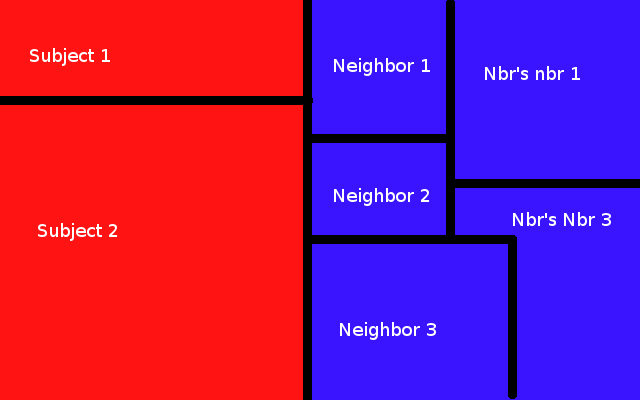
\includegraphics[scale = 0.5]{../analysis/output/borders_temp.png}
    \caption{Red rectangles are subject counties, and blue are neighbor counties. In this example Subject 1 would be only matched to Neighbor 1, while "Subject 2" would be paired with Neighbor 1-3. Similarly, when we broaden the bandwidth, Subject 1 would be matched with Nbr's Nbr 1, whle Subject 2 would be paired with Nbr's Nbr 1 and 2}
\end{figure}

\begin{figure}[h]\label{eb}
    \centering
    \textbf{Original Bandwidth Borders}\par\medskip
    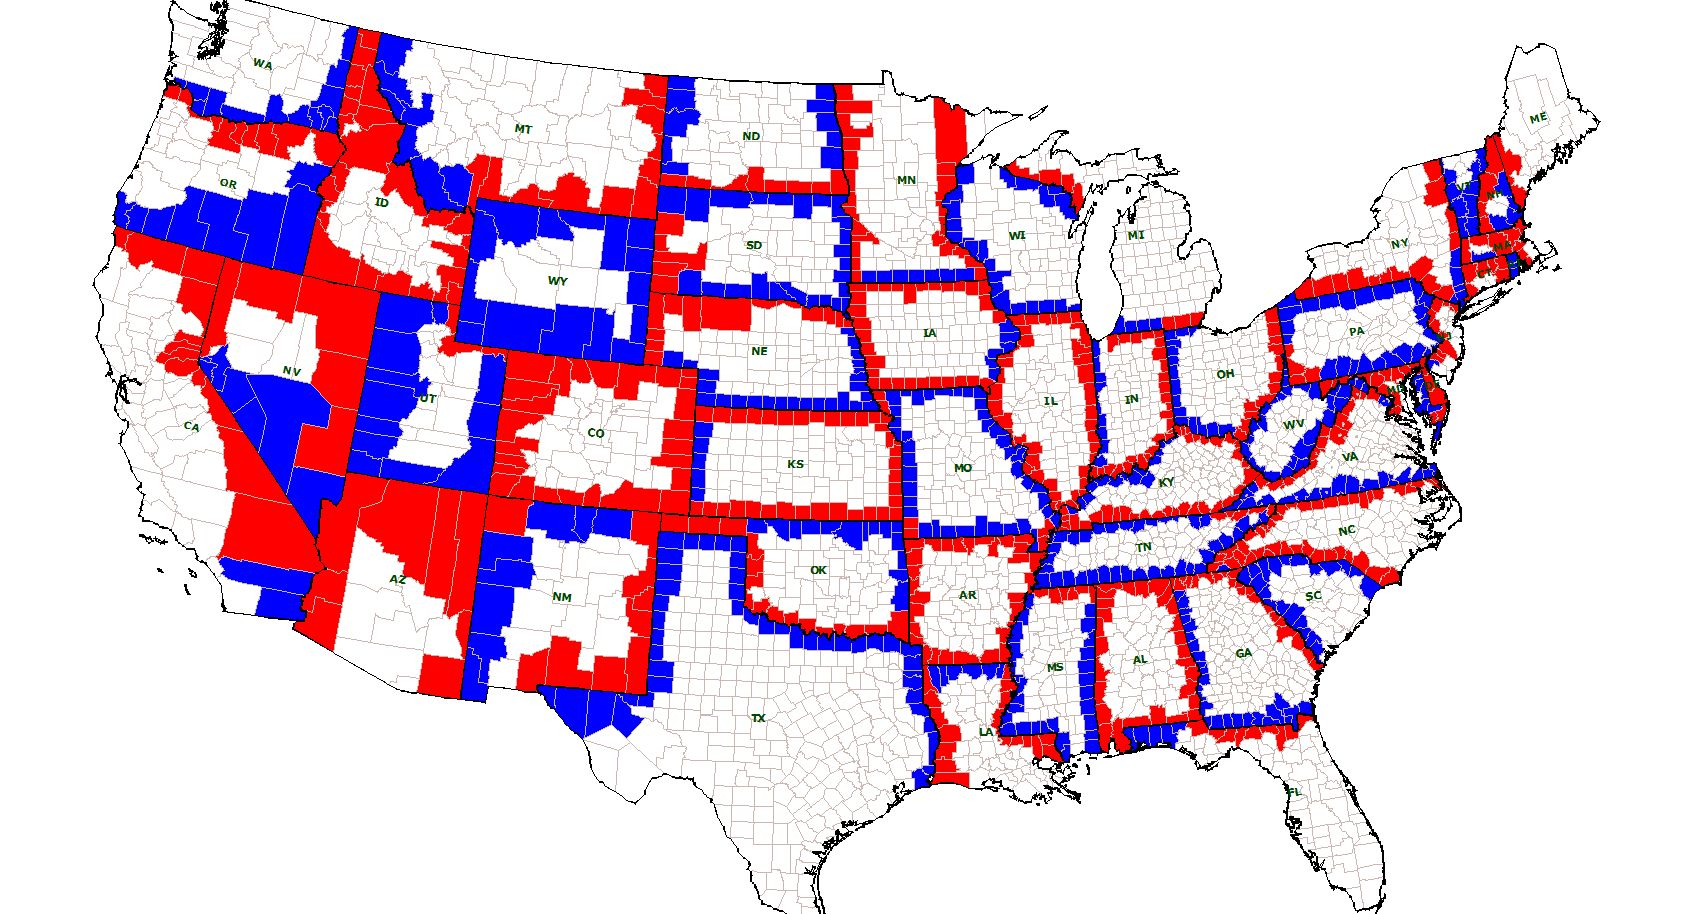
\includegraphics[scale = 0.20]{../analysis/output/rb_picture.png}
    \caption{Red borders are subject counties, blue borders are neighbor counties}
\end{figure}

\begin{figure}[h]
    \centering
    \textbf{Extended Bandwidth Borders}\par\medskip
    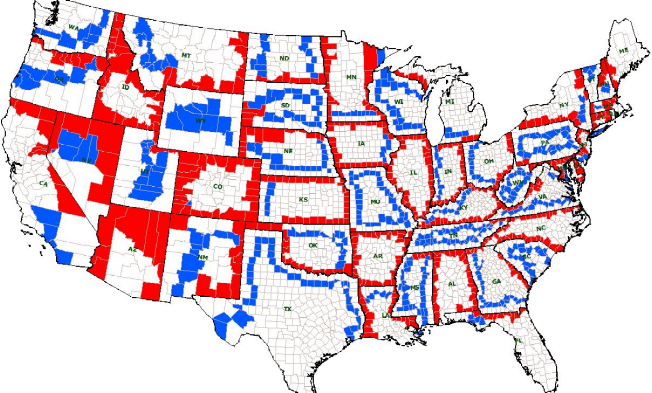
\includegraphics[scale = 0.5]{../analysis/output/eb_picture.png}
    \caption{Red borders are subject counties, blue borders are neighbor counties}
\end{figure}


% Table created by stargazer v.5.2 by Marek Hlavac, Harvard University. E-mail: hlavac at fas.harvard.edu
% Date and time: Tue, Apr 19, 2016 - 09:24:57 AM
\begin{table}[!htbp] \centering 
  \caption{Summary Table for  Total Firm Births} 
  \label{--summary} 
\begin{tabular}{@{\extracolsep{5pt}}lccccc} 
\\[-1.8ex]\hline 
\hline \\[-1.8ex] 
Statistic & \multicolumn{1}{c}{N} & \multicolumn{1}{c}{Mean} & \multicolumn{1}{c}{St. Dev.} & \multicolumn{1}{c}{Min} & \multicolumn{1}{c}{Max} \\ 
\hline \\[-1.8ex] 
Births Ratio & 13,115 & $-$0.059 & 1.550 & $-$5.670 & 5.328 \\ 
Property Tax Difference & 13,115 & $-$0.099 & 0.503 & $-$1.672 & 1.241 \\ 
Income Tax Difference & 13,115 & 1.220 & 3.988 & $-$9.280 & 9.860 \\ 
Capital Gains Tax Difference & 13,115 & 1.911 & 4.321 & $-$9.280 & 13.420 \\ 
Sales Tax Difference & 13,115 & $-$0.316 & 2.137 & $-$7.000 & 7.250 \\ 
Corp Tax Difference & 13,115 & 1.282 & 3.678 & $-$8.900 & 12.000 \\ 
Workers Comp Tax Difference & 13,115 & 0.030 & 0.666 & $-$2.762 & 2.451 \\ 
Unemp. Tax Difference & 13,115 & 0.034 & 1.344 & $-$4.564 & 16.070 \\ 
Educ Spending Per Cap Diff & 13,115 & 9.589 & 210.233 & $-$807 & 692 \\ 
Highway Spending Per Cap Diff & 13,115 & $-$39.025 & 144.832 & $-$756 & 358 \\ 
Welfare Spending Per Cap Diff & 13,115 & $-$38.699 & 267.490 & $-$1,072 & 953 \\ 
Pct Highschool & 13,115 & 0.273 & 3.762 & $-$10.100 & 12.000 \\ 
Real Fuel Price & 13,115 & 0.306 & 2.351 & $-$7.500 & 8.200 \\ 
Pct Union & 13,115 & 0.636 & 4.672 & $-$14.900 & 16.100 \\ 
Pop Density & 13,115 & 41.985 & 162.362 & $-$746.200 & 901.000 \\ 
Pct Manuf & 13,115 & 0.011 & 0.067 & $-$0.240 & 0.250 \\ 
Jan Temp Z Diff & 13,115 & 0.002 & 0.206 & $-$1.291 & 1.291 \\ 
Jan Sun Z Diff & 13,115 & 0.042 & 0.582 & $-$2.499 & 3.583 \\ 
Jul Temp Z Diff & 13,115 & 0.065 & 0.601 & $-$4.475 & 4.115 \\ 
Jul Hum Z Diff & 13,115 & $-$0.029 & 0.424 & $-$3.697 & 3.081 \\ 
Topog Z Diff & 13,115 & $-$0.023 & 0.645 & $-$2.578 & 2.123 \\ 
Ln Water Z Diff & 13,115 & $-$0.054 & 0.872 & $-$3.456 & 3.155 \\ 
\hline \\[-1.8ex] 
\multicolumn{6}{l}{All variables are for the difference between our subject and neighbor counties. At the state level, this is 1177 observations. Further, all tax variables are scaled to be between 0 and 100 rather than 0 and 1. For each variable we observe them 13,115 times when not accounting for positive or negative infinify values in firm start up rates.} \\ 
\end{tabular} 
\end{table} 


\begin{figure}[h]\label{pairs}
    \centering
    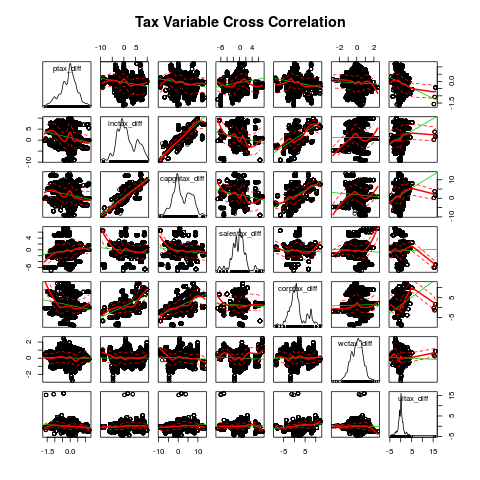
\includegraphics[scale = 0.5]{../analysis/output/_--_pairs.png}
\end{figure}

\newgeometry{margin=1cm}
\begin{landscape}

% Table created by stargazer v.5.2 by Marek Hlavac, Harvard University. E-mail: hlavac at fas.harvard.edu
% Date and time: Sat, Sep 03, 2016 - 06:49:03 AM
\begin{table}[!htbp] \centering 
  \caption{Regression Discontinuity Models for  Total Firm Births} 
  \label{--rd} 
\footnotesize 
\begin{tabular}{@{\extracolsep{5pt}}lcccccc} 
\\[-1.8ex]\hline 
\hline \\[-1.8ex] 
 & \multicolumn{6}{c}{\textit{Dependent variable:}} \\ 
\cline{2-7} 
\\[-1.8ex] & \multicolumn{6}{c}{births ratio} \\ 
 & OLS & OLS & OLS & OLS & FE & FE \\ 
\\[-1.8ex] & (1) & (2) & (3) & (4) & (5) & (6)\\ 
\hline \\[-1.8ex] 
 Property Tax Difference & $-$0.199 & $-$0.363$^{**}$ & $-$0.129 & $-$0.291$^{*}$ & $-$0.008 & $-$0.020 \\ 
  & (0.151) & (0.147) & (0.148) & (0.150) & (0.120) & (0.123) \\ 
  Income Tax Difference & $-$0.094$^{***}$ & $-$0.086$^{***}$ & $-$0.088$^{***}$ & $-$0.076$^{***}$ & $-$0.024 & $-$0.023 \\ 
  & (0.027) & (0.025) & (0.028) & (0.026) & (0.035) & (0.035) \\ 
  Capital Gains Tax Difference & 0.017 & 0.009 & 0.028 & 0.019 & 0.0001 & 0.001 \\ 
  & (0.023) & (0.023) & (0.024) & (0.024) & (0.012) & (0.013) \\ 
  Sales Tax Difference & $-$0.117$^{***}$ & $-$0.106$^{***}$ & $-$0.112$^{***}$ & $-$0.089$^{***}$ & 0.005 & 0.004 \\ 
  & (0.029) & (0.029) & (0.028) & (0.031) & (0.040) & (0.041) \\ 
  Corp Tax Difference & 0.023 & 0.018 & 0.015 & 0.011 & $-$0.008 & $-$0.008 \\ 
  & (0.020) & (0.018) & (0.020) & (0.019) & (0.026) & (0.026) \\ 
  Workers Comp Tax Difference & 0.009 & 0.095 & $-$0.001 & 0.055 & 0.022 & 0.021 \\ 
  & (0.111) & (0.107) & (0.095) & (0.104) & (0.069) & (0.071) \\ 
  Unemp. Tax Difference & 0.009 & 0.013 & $-$0.002 & $-$0.005 & $-$0.001 & $-$0.002 \\ 
  & (0.041) & (0.037) & (0.044) & (0.039) & (0.018) & (0.019) \\ 
  Educ Spending Per Cap Diff & $-$0.0002 & $-$0.0002 & $-$0.0001 & $-$0.0002 & $-$0.0002 & $-$0.0001 \\ 
  & (0.0002) & (0.0003) & (0.0003) & (0.0003) & (0.0002) & (0.0002) \\ 
  Highway Spending Per Cap Diff & 0.0004 & 0.0004 & 0.0002 & 0.0003 & 0.0001 & 0.0001 \\ 
  & (0.0004) & (0.0004) & (0.0004) & (0.0004) & (0.0002) & (0.0002) \\ 
  Welfare Spending Per Cap Diff & 0.001$^{**}$ & 0.001$^{**}$ & 0.001$^{**}$ & 0.0004$^{*}$ & $-$0.0001 & $-$0.0001 \\ 
  & (0.0002) & (0.0003) & (0.0003) & (0.0003) & (0.0001) & (0.0001) \\ 
  Constant & $-$0.053 & $-$0.064 & $-$0.041 & $-$0.051 &  &  \\ 
  & (0.084) & (0.085) & (0.087) & (0.086) &  &  \\ 
 \hline \\[-1.8ex] 
controls & Yes & Yes & No & No & Yes & Yes \\ 
amenities & Yes & No & Yes & No & Yes & No \\ 
\hline \\[-1.8ex] 
Observations & 13,042 & 13,042 & 13,042 & 13,042 & 13,042 & 13,042 \\ 
R$^{2}$ & 0.094 & 0.055 & 0.080 & 0.037 & 0.243 & 0.205 \\ 
\hline 
\hline \\[-1.8ex] 
\textit{Note:}  & \multicolumn{6}{r}{$^{*}$p$<$0.1; $^{**}$p$<$0.05; $^{***}$p$<$0.01} \\ 
 & \multicolumn{6}{r}{The first four columns are estimated with OLS and clustered standard} \\ 
 & \multicolumn{6}{r}{ errors at the state-pair level. Columns 5 and 6 are estimated with} \\ 
 & \multicolumn{6}{r}{a fixed effect estimator at the state-pair level with homoskedastic} \\ 
 & \multicolumn{6}{r}{standard errors.} \\ 
\end{tabular} 
\end{table} 

\end{landscape}
\restoregeometry

\newgeometry{margin=1cm}
\begin{landscape}

% Table created by stargazer v.5.2 by Marek Hlavac, Harvard University. E-mail: hlavac at fas.harvard.edu
% Date and time: Fri, Jan 15, 2016 - 10:30:13 AM
\begin{table}[!htbp] \centering 
  \caption{Extended Bandwidth Discontinuity Models for  Total Firm Births} 
  \label{--rd} 
\begin{tabular}{@{\extracolsep{5pt}}lcccccc} 
\\[-1.8ex]\hline 
\hline \\[-1.8ex] 
 & \multicolumn{6}{c}{\textit{Dependent variable:}} \\ 
\cline{2-7} 
\\[-1.8ex] & \multicolumn{6}{c}{births ratio} \\ 
 & OLS & OLS & OLS & OLS & FE & FE \\ 
\\[-1.8ex] & (1) & (2) & (3) & (4) & (5) & (6)\\ 
\hline \\[-1.8ex] 
 Property Tax Difference & 0.039 & $-$0.019 & 0.104 & 0.074 & 0.007 & 0.006 \\ 
  & (0.147) & (0.152) & (0.143) & (0.148) & (0.112) & (0.114) \\ 
  Income Tax Difference & $-$0.054 & $-$0.063$^{*}$ & $-$0.043 & $-$0.050 & 0.008 & 0.012 \\ 
  & (0.035) & (0.036) & (0.038) & (0.037) & (0.033) & (0.034) \\ 
  Capital Gains Tax Difference & 0.039 & 0.048$^{*}$ & 0.043 & 0.053$^{*}$ & $-$0.013 & $-$0.013 \\ 
  & (0.029) & (0.028) & (0.033) & (0.030) & (0.012) & (0.012) \\ 
  Sales Tax Difference & $-$0.040 & $-$0.042 & $-$0.051 & $-$0.041 & 0.018 & 0.020 \\ 
  & (0.049) & (0.054) & (0.052) & (0.055) & (0.037) & (0.038) \\ 
  Corp Tax Difference & 0.006 & $-$0.001 & 0.004 & 0.002 & $-$0.024 & $-$0.024 \\ 
  & (0.026) & (0.025) & (0.027) & (0.025) & (0.024) & (0.024) \\ 
  Workers Comp Tax Difference & 0.180 & 0.300$^{**}$ & 0.139 & 0.216 & $-$0.008 & $-$0.007 \\ 
  & (0.126) & (0.152) & (0.142) & (0.178) & (0.066) & (0.068) \\ 
  Unemp. Tax Difference & $-$0.113$^{*}$ & $-$0.110$^{*}$ & $-$0.111 & $-$0.109 & 0.011 & 0.011 \\ 
  & (0.062) & (0.064) & (0.068) & (0.071) & (0.018) & (0.019) \\ 
  Educ Spending Per Cap Diff & 0.0001 & 0.0002 & 0.0002 & 0.0003 & $-$0.0001 & $-$0.0001 \\ 
  & (0.0005) & (0.001) & (0.0005) & (0.001) & (0.0002) & (0.0002) \\ 
  Highway Spending Per Cap Diff & 0.0002 & 0.0001 & $-$0.0002 & $-$0.0003 & 0.0001 & 0.00005 \\ 
  & (0.0005) & (0.001) & (0.0005) & (0.001) & (0.0002) & (0.0002) \\ 
  Welfare Spending Per Cap Diff & 0.001 & 0.001$^{*}$ & 0.001$^{*}$ & 0.001$^{*}$ & $-$0.00003 & $-$0.00004 \\ 
  & (0.0004) & (0.0004) & (0.0004) & (0.0004) & (0.0001) & (0.0001) \\ 
  Constant & $-$0.033 & $-$0.017 & $-$0.026 & 0.002 &  &  \\ 
  & (0.100) & (0.111) & (0.105) & (0.113) &  &  \\ 
 \hline \\[-1.8ex] 
controls & Yes & Yes & No & No & Yes & Yes \\ 
amenities & Yes & No & Yes & No & Yes & No \\ 
\hline \\[-1.8ex] 
Observations & 16,245 & 16,245 & 16,245 & 16,245 & 16,245 & 16,245 \\ 
R$^{2}$ & 0.097 & 0.038 & 0.081 & 0.023 & 0.298 & 0.267 \\ 
\hline 
\hline \\[-1.8ex] 
\textit{Note:}  & \multicolumn{6}{r}{$^{*}$p$<$0.1; $^{**}$p$<$0.05; $^{***}$p$<$0.01} \\ 
\end{tabular} 
\end{table} 

\end{landscape}
\restoregeometry


% Table created by stargazer v.5.2 by Marek Hlavac, Harvard University. E-mail: hlavac at fas.harvard.edu
% Date and time: Tue, Apr 05, 2016 - 11:02:14 AM
\begin{table}[!htbp] \centering 
  \caption{Not Symmetric Effects for  Total Firm Births} 
  \label{--noequality} 
\footnotesize 
\begin{tabular}{@{\extracolsep{5pt}}lcc} 
\\[-1.8ex]\hline 
\hline \\[-1.8ex] 
 & \multicolumn{2}{c}{\textit{Dependent variable:}} \\ 
\cline{2-3} 
\\[-1.8ex] & \multicolumn{2}{c}{births ratio} \\ 
 & OLS & OLS \\ 
\\[-1.8ex] & (1) & (2)\\ 
\hline \\[-1.8ex] 
 Property Tax Sub & $-$0.048 & $-$0.363$^{**}$ \\ 
  & (0.185) & (0.172) \\ 
  Property Tax Nbr & 0.209 & 0.352$^{**}$ \\ 
  & (0.162) & (0.148) \\ 
  Income Tax Sub & $-$0.149$^{***}$ & $-$0.125$^{***}$ \\ 
  & (0.053) & (0.044) \\ 
  Income Tax Nbr & 0.076$^{*}$ & 0.057$^{*}$ \\ 
  & (0.039) & (0.032) \\ 
  Capital Gains Tax Sub & 0.037 & 0.025 \\ 
  & (0.034) & (0.031) \\ 
  Capital Gains Tax nbr & $-$0.069$^{**}$ & $-$0.047 \\ 
  & (0.034) & (0.031) \\ 
  Sales Tax Sub & $-$0.149$^{***}$ & $-$0.142$^{***}$ \\ 
  & (0.044) & (0.041) \\ 
  Sales Tax Nbr & 0.036 & 0.005 \\ 
  & (0.045) & (0.045) \\ 
  Corp Tax Sub & 0.026 & 0.029 \\ 
  & (0.028) & (0.027) \\ 
  Corp Tax Nbr & 0.011 & 0.001 \\ 
  & (0.023) & (0.024) \\ 
  Workers Comp Tax Sub & $-$0.142 & $-$0.113 \\ 
  & (0.131) & (0.120) \\ 
  Workers Comp Tax Nbr & $-$0.122 & $-$0.226 \\ 
  & (0.149) & (0.150) \\ 
  Unemp. Tax Sub & $-$0.018 & $-$0.059 \\ 
  & (0.043) & (0.044) \\ 
  Unemp. Tax Nbr & $-$0.014 & $-$0.023 \\ 
  & (0.076) & (0.057) \\ 
  Educ Spending Per Cap Sub & $-$0.0001 & $-$0.001 \\ 
  & (0.0004) & (0.0004) \\ 
  Educ Spending Per Cap Nbr & 0.0002 & 0.0001 \\ 
  & (0.0004) & (0.0004) \\ 
  Highway Spending Per Cap Sub & 0.0004 & 0.001 \\ 
  & (0.001) & (0.001) \\ 
  Highway Spending Per Cap Nbr & $-$0.001 & $-$0.0004 \\ 
  & (0.001) & (0.001) \\ 
  Welfare Spending Per Cap Sub & 0.001$^{**}$ & 0.001$^{**}$ \\ 
  & (0.0003) & (0.0003) \\ 
  Welfare Spending Per Cap Sub & $-$0.0005 & $-$0.0003 \\ 
  & (0.0003) & (0.0003) \\ 
  Constant & 1.085 & 1.667$^{**}$ \\ 
  & (0.863) & (0.764) \\ 
 \hline \\[-1.8ex] 
amenities & Yes & No \\ 
\hline \\[-1.8ex] 
Observations & 13,115 & 13,115 \\ 
R$^{2}$ & 0.098 & 0.053 \\ 
\hline 
\hline \\[-1.8ex] 
\textit{Note:}  & \multicolumn{2}{r}{$^{*}$p$<$0.1; $^{**}$p$<$0.05; $^{***}$p$<$0.01} \\ 
 & \multicolumn{2}{r}{Each model is estimated with Ordinary Least Squares} \\ 
 & \multicolumn{2}{r}{with clustered standard errors at the state-pair level.} \\ 
 & \multicolumn{2}{r}{coefficient values and standard errors are reported.} \\ 
\end{tabular} 
\end{table} 


% Table created by stargazer v.5.2 by Marek Hlavac, Harvard University. E-mail: hlavac at fas.harvard.edu
% Date and time: Fri, Jan 15, 2016 - 10:30:04 AM
\begin{table}[!htbp] \centering 
  \caption{F-Tests for Symmetry of Coefficients for Total Firm Start Ups} 
  \label{--Ftests} 
\begin{tabular}{@{\extracolsep{5pt}} ccc} 
\\[-1.8ex]\hline 
\hline \\[-1.8ex] 
Test & F-Stat & P(\textgreater F) \\ 
\hline \\[-1.8ex] 
ptax\_sub = -ptax\_nbr & 0.0064 & 0.9361 \\ 
inctax\_sub = -inctax\_nbr & 1.7426 & 0.1868 \\ 
capgntax\_sub = -capgntax\_nbr & 0.3873 & 0.5337 \\ 
salestax\_sub = -salestax\_nbr & 4.5658 & 0.0326 \\ 
corptax\_sub = -corptax\_nbr & 0.6824 & 0.4088 \\ 
wctaxfixed\_sub = -wctaxfixed\_nbr & 3.2369 & 0.072 \\ 
uitaxrate\_sub = -uitaxrate\_nbr & 1.8872 & 0.1695 \\ 
\hline \\[-1.8ex] 
\end{tabular} 
\end{table} 


\newgeometry{margin=1cm}
\begin{landscape}

% Table created by stargazer v.5.2 by Marek Hlavac, Harvard University. E-mail: hlavac at fas.harvard.edu
% Date and time: Fri, Jan 15, 2016 - 10:30:09 AM
\begin{table}[!htbp] \centering 
  \caption{Psuedo-RD for Stability over Time for  Total Firm Births} 
  \label{--year} 
\small 
\begin{tabular}{@{\extracolsep{5pt}}lccccccccccc} 
\\[-1.8ex]\hline 
\hline \\[-1.8ex] 
 & \multicolumn{11}{c}{\textit{Dependent variable:}} \\ 
\cline{2-12} 
\\[-1.8ex] & \multicolumn{11}{c}{births ratio} \\ 
 & 1999 & 2000 & 2001 & 2002 & 2003 & 2004 & 2005 & 2006 & 2007 & 2008 & 2009 \\ 
\\[-1.8ex] & (1) & (2) & (3) & (4) & (5) & (6) & (7) & (8) & (9) & (10) & (11)\\ 
\hline \\[-1.8ex] 
 Prop Tax Diff & $-$0.411 & $-$0.371 & $-$0.426 & $-$0.390 & $-$0.320 & $-$0.479 & $-$0.344 & $-$0.364 & $-$0.396 & $-$0.311 & $-$0.351$^{***}$ \\ 
  & ($-$0.411) & ($-$0.426) & ($-$0.390) & ($-$0.320) & ($-$0.479) & ($-$0.344) & ($-$0.364) & ($-$0.396) & ($-$0.311) & ($-$0.351) & (0.116) \\ 
  Inc Tax Diff & $-$0.025 & $-$0.026 & $-$0.066 & $-$0.061 & $-$0.047 & $-$0.055 & $-$0.063 & $-$0.136 & $-$0.127 & $-$0.123 & $-$0.117$^{***}$ \\ 
  & ($-$0.025) & ($-$0.066) & ($-$0.061) & ($-$0.047) & ($-$0.055) & ($-$0.063) & ($-$0.136) & ($-$0.127) & ($-$0.123) & ($-$0.117) & (0.026) \\ 
  Cap Tax Diff & $-$0.045 & $-$0.040 & $-$0.025$^{***}$ & $-$0.006 & $-$0.018 & $-$0.032 & $-$0.029 & 0.054 & 0.036 & 0.032 & 0.028 \\ 
  & ($-$0.045) & ($-$0.025) & ($-$0.006) & ($-$0.018) & ($-$0.032) & ($-$0.029) & (0.054) & (0.036) & (0.032) & (0.028) & (0.023) \\ 
  Sal Tax Diff & $-$0.083 & $-$0.097 & $-$0.104 & $-$0.106 & $-$0.095 & $-$0.119 & $-$0.136 & $-$0.102 & $-$0.110 & $-$0.140 & $-$0.132$^{***}$ \\ 
  & ($-$0.083) & ($-$0.104) & ($-$0.106) & ($-$0.095) & ($-$0.119) & ($-$0.136) & ($-$0.102) & ($-$0.110) & ($-$0.140) & ($-$0.132) & (0.026) \\ 
  Corp Tax Diff & $-$0.015 & 0.011 & 0.010 & 0.007 & 0.035 & 0.030 & 0.037$^{*}$ & 0.019$^{***}$ & 0.004 & 0.014$^{**}$ & $-$0.007 \\ 
  & ($-$0.015) & (0.010) & (0.007) & (0.035) & (0.030) & (0.037) & (0.019) & (0.004) & (0.014) & ($-$0.007) & (0.018) \\ 
  Work Comp Diff & 0.309 & 0.225 & 0.201$^{***}$ & 0.018 & 0.029 & 0.071 & 0.066 & 0.142 & 0.102 & 0.086 & 0.089 \\ 
  & (0.309) & (0.201) & (0.018) & (0.029) & (0.071) & (0.066) & (0.142) & (0.102) & (0.086) & (0.089) & (0.092) \\ 
  Unemp. Tax Diff & $-$0.045 & 0.0001 & 0.015 & 0.027 & $-$0.022 & 0.062$^{***}$ & 0.003 & $-$0.014 & $-$0.034$^{*}$ & 0.020 & 0.070$^{*}$ \\ 
  & ($-$0.045) & (0.015) & (0.027) & ($-$0.022) & (0.062) & (0.003) & ($-$0.014) & ($-$0.034) & (0.020) & (0.070) & (0.039) \\ 
  Ln Educ Diff & $-$0.0001 & $-$0.0002 & $-$0.0003 & $-$0.0002 & $-$0.0002 & $-$0.001$^{**}$ & $-$0.0003$^{***}$ & 0.0001 & $-$0.0002 & $-$0.0001 & $-$0.0002 \\ 
  & ($-$0.0001) & ($-$0.0003) & ($-$0.0002) & ($-$0.0002) & ($-$0.001) & ($-$0.0003) & (0.0001) & ($-$0.0002) & ($-$0.0001) & ($-$0.0002) & (0.0002) \\ 
  Ln Hwy Diff & 0.001 & 0.002 & 0.001$^{***}$ & 0.0002 & 0.0004 & 0.0004$^{***}$ & 0.0001 & 0.0002$^{*}$ & 0.0001 & $-$0.0002 & $-$0.0004 \\ 
  & (0.001) & (0.001) & (0.0002) & (0.0004) & (0.0004) & (0.0001) & (0.0002) & (0.0001) & ($-$0.0002) & ($-$0.0004) & (0.0003) \\ 
  Ln Welf. Diff & 0.001 & 0.001 & 0.001 & 0.001 & 0.001 & 0.0005 & 0.001 & 0.001 & 0.001 & 0.001 & 0.001$^{***}$ \\ 
  & (0.001) & (0.001) & (0.001) & (0.001) & (0.0005) & (0.001) & (0.001) & (0.001) & (0.001) & (0.001) & (0.0002) \\ 
  Constant & $-$0.034 & $-$0.026$^{*}$ & $-$0.013 & $-$0.057$^{***}$ & 0.007 & $-$0.042$^{***}$ & $-$0.015 & $-$0.097 & $-$0.072 & $-$0.086 & $-$0.075 \\ 
  & ($-$0.034) & ($-$0.013) & ($-$0.057) & (0.007) & ($-$0.042) & ($-$0.015) & ($-$0.097) & ($-$0.072) & ($-$0.086) & ($-$0.075) & (0.056) \\ 
 \hline \\[-1.8ex] 
controls & Yes & Yes & Yes & Yes & Yes & Yes & Yes & Yes & Yes & Yes & Yes \\ 
amenities & No & No & No & No & No & No & No & No & No & No & No \\ 
\hline \\[-1.8ex] 
Observations & 1,193 & 1,188 & 1,191 & 1,195 & 1,189 & 1,188 & 1,191 & 1,194 & 1,199 & 1,196 & 1,191 \\ 
R$^{2}$ & 0.068 & 0.059 & 0.066 & 0.050 & 0.052 & 0.068 & 0.064 & 0.062 & 0.069 & 0.067 & 0.077 \\ 
\hline 
\hline \\[-1.8ex] 
\textit{Note:}  & \multicolumn{11}{r}{$^{*}$p$<$0.1; $^{**}$p$<$0.05; $^{***}$p$<$0.01} \\ 
\end{tabular} 
\end{table} 

\end{landscape}
\restoregeometry

\newgeometry{margin=1cm}
\begin{landscape}

% Table created by stargazer v.5.2 by Marek Hlavac, Harvard University. E-mail: hlavac at fas.harvard.edu
% Date and time: Mon, Feb 15, 2016 - 10:02:27 AM
\begin{table}[!htbp] \centering 
  \caption{Results for Firm Entry across NAICS Subcodes for } 
  \label{naics} 
\small 
\begin{tabular}{@{\extracolsep{5pt}}lcccccccc} 
\\[-1.8ex]\hline 
\hline \\[-1.8ex] 
 & \multicolumn{8}{c}{\textit{Dependent variable:}} \\ 
\cline{2-9} 
\\[-1.8ex] & \multicolumn{8}{c}{births ratio} \\ 
 & Farming & Farming & Manuf & Manuf & Retail & Retail & Finance & Finance \\ 
\\[-1.8ex] & (1) & (2) & (3) & (4) & (5) & (6) & (7) & (8)\\ 
\hline \\[-1.8ex] 
 Property Tax Difference & $-$0.035 & 0.058 & $-$0.037 & 0.054 & $-$0.003 & 0.087 & $-$0.025 & 0.066 \\ 
  & ($-$0.035) & (0.058) & ($-$0.037) & (0.054) & ($-$0.003) & (0.087) & ($-$0.025) & (0.066) \\ 
  Income Tax Difference & $-$0.061 & $-$0.048 & $-$0.062 & $-$0.049 & $-$0.061 & $-$0.049 & $-$0.060 & $-$0.047 \\ 
  & ($-$0.061) & ($-$0.048) & ($-$0.062) & ($-$0.049) & ($-$0.061) & ($-$0.049) & ($-$0.060) & ($-$0.047) \\ 
  Capital Gains Tax Difference & 0.045 & 0.051 & 0.047 & 0.052 & 0.045 & 0.051 & 0.044 & 0.050 \\ 
  & (0.045) & (0.051) & (0.047) & (0.052) & (0.045) & (0.051) & (0.044) & (0.050) \\ 
  Sales Tax Difference & $-$0.042 & $-$0.041 & $-$0.038 & $-$0.037 & $-$0.043 & $-$0.042 & $-$0.038 & $-$0.038 \\ 
  & ($-$0.042) & ($-$0.041) & ($-$0.038) & ($-$0.037) & ($-$0.043) & ($-$0.042) & ($-$0.038) & ($-$0.038) \\ 
  Corp Tax Difference & 0.001 & 0.003 & 0.002 & 0.005 & 0.001 & 0.003 & 0.001 & 0.004 \\ 
  & (0.001) & (0.003) & (0.002) & (0.005) & (0.001) & (0.003) & (0.001) & (0.004) \\ 
  Workers Comp Tax Difference & 0.283 & 0.204 & 0.298 & 0.213 & 0.290 & 0.215 & 0.300 & 0.213 \\ 
  & (0.283) & (0.204) & (0.298) & (0.213) & (0.290) & (0.215) & (0.300) & (0.213) \\ 
  Unemp. Tax Difference & $-$0.106 & $-$0.109 & $-$0.108 & $-$0.110 & $-$0.109 & $-$0.111 & $-$0.106 & $-$0.107 \\ 
  & ($-$0.106) & ($-$0.109) & ($-$0.108) & ($-$0.110) & ($-$0.109) & ($-$0.111) & ($-$0.106) & ($-$0.107) \\ 
  Educ Spending Per Cap Diff & 0.0002 & 0.0003 & 0.0002 & 0.0003 & 0.0003 & 0.0003 & 0.0002 & 0.0003 \\ 
  & (0.0002) & (0.0003) & (0.0002) & (0.0003) & (0.0003) & (0.0003) & (0.0002) & (0.0003) \\ 
  Highway Spending Per Cap Diff & 0.0001 & $-$0.0003 & 0.0001 & $-$0.0003 & 0.0001 & $-$0.0003 & 0.0001 & $-$0.0003 \\ 
  & (0.0001) & ($-$0.0003) & (0.0001) & ($-$0.0003) & (0.0001) & ($-$0.0003) & (0.0001) & ($-$0.0003) \\ 
  Welfare Spending Per Cap Diff & 0.001 & 0.001 & 0.001 & 0.001 & 0.001 & 0.001 & 0.001 & 0.001 \\ 
  & (0.001) & (0.001) & (0.001) & (0.001) & (0.001) & (0.001) & (0.001) & (0.001) \\ 
  Constant & $-$0.020 & $-$0.002 & $-$0.024 & $-$0.009 & $-$0.014 & 0.002 & $-$0.016 & $-$0.0005 \\ 
  & ($-$0.020) & ($-$0.002) & ($-$0.024) & ($-$0.009) & ($-$0.014) & (0.002) & ($-$0.016) & ($-$0.0005) \\ 
 \hline \\[-1.8ex] 
controls & Yes & No & Yes & No & Yes & No & Yes & No \\ 
amenities & No & No & No & No & No & No & No & No \\ 
\hline \\[-1.8ex] 
Observations & 15,084 & 15,084 & 15,609 & 15,609 & 16,081 & 16,081 & 15,582 & 15,582 \\ 
R$^{2}$ & 0.038 & 0.023 & 0.037 & 0.023 & 0.037 & 0.023 & 0.036 & 0.022 \\ 
\hline 
\hline \\[-1.8ex] 
\textit{Note:}  & \multicolumn{8}{r}{$^{*}$p$<$0.1; $^{**}$p$<$0.05; $^{***}$p$<$0.01} \\ 
 & \multicolumn{8}{r}{All models are estimated with Ordinary Least Squares and clustered standard errors at the state-pair level.} \\ 
\end{tabular} 
\end{table} 

\end{landscape}
\restoregeometry

\begin{figure}[h]\label{weightedtax}
    \centering
    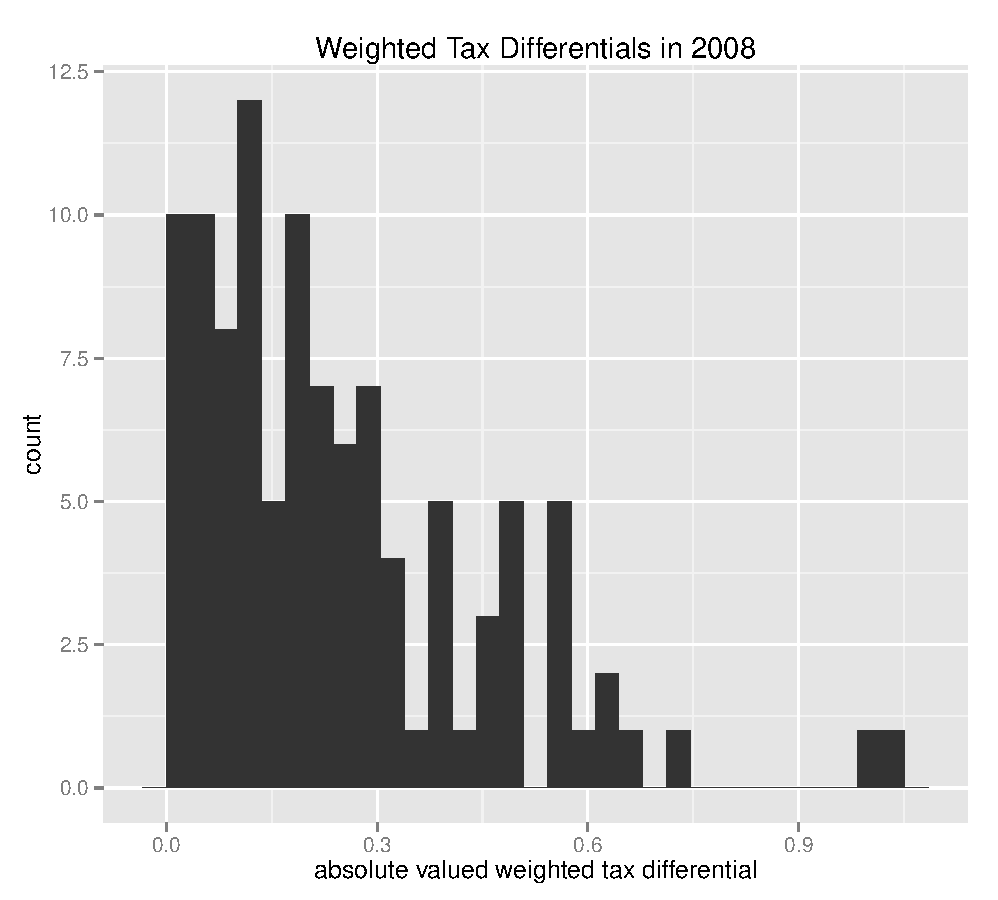
\includegraphics[scale = 0.5]{../analysis/output/_--_weightedtax.pdf}
\end{figure}


% Table created by stargazer v.5.2 by Marek Hlavac, Harvard University. E-mail: hlavac at fas.harvard.edu
% Date and time: Mon, Feb 15, 2016 - 03:01:17 PM
\begin{table}[!htbp] \centering 
  \caption{Result Comparison for Total Firm Births} 
  \label{meantable} 
\tiny 
\begin{tabular}{@{\extracolsep{5pt}} ccccccc} 
\\[-1.8ex]\hline 
\hline \\[-1.8ex] 
mean firm entry & preffered side & abs weighted tax & preferred side & same? & sub state & nbr state \\ 
\hline \\[-1.8ex] 
$2.591$ & nbr & $0.010$ & sub & different & kansas & nebraska \\ 
$2.260$ & nbr & $0.016$ & nbr & same & maryland & west virginia \\ 
$2.194$ & sub & $0.294$ & sub & same & alabama & georgia \\ 
$2.126$ & sub & $0.205$ & nbr & different & minnesota & wisconsin \\ 
$1.808$ & sub & $0.097$ & nbr & different & ohio & pennsylvania \\ 
$1.743$ & sub & $0.555$ & sub & same & colorado & kansas \\ 
$1.568$ & nbr & $0.105$ & nbr & same & arizona & nevada \\ 
$1.513$ & nbr & $0.256$ & sub & different & idaho & utah \\ 
$1.477$ & sub & $0.119$ & sub & same & oklahoma & texas \\ 
$1.376$ & nbr & $0.015$ & nbr & same & kentucky & west virginia \\ 
\hline \\[-1.8ex] 
\end{tabular} 
\end{table} 


\end{document}